\chapter{Resultados}

\section{Resultados del cálculo de combustión}
\par Los resultados para el cálculo de combustión, con los datos de las Tabla \ref{tbl:combustible} y \ref{tbl:aire}, se muestran en la Tabla \ref{tbl:combustion-data}. La composición del gas de combustión resultante se describe en la Tabla \ref{tbl:combustion-gas}.
\begin{table}[hbt]
\begin{center}
\caption[Resultados de la combustión simulada]{Resultados de la combustión simulada.}
\label{tbl:combustion-data}
\begin{tabular}{l|c}
	A/C másica teórica requerido					& 15.574 \\
	A/C másica húmeda con exceso de aire			& 18.689 \\
	Unidad de gas de combustión por unidad de aire  & 19.689 \\
	Poder Calorífico Neto  (NCV), kJ/kg				& 45,718.6 \\
	Poder Calorífico Bruto (GCV), kJ/kg				& 50,268.0 \\
	Peso Molecular (PM) del combustible, kg/kmol	& 21.149 \\
	PM del gas de combustión, kg/kmol				& 27.911 \\
\end{tabular}
\end{center}
\end{table}
\par Para validar la confiabilidad de estos resultados se compararon con los obtenidos en el software privado de diseño de hornos, WinHeat\copyright, utilizado para evaluación térmica y análisis de hornos de fuego directo, propiedad de Esteem Projects Pvt. Ltd., con una licencia autorizada para la versión 3.0. La conclusión de esta comparación arrojó que la diferencia entre los resultados de ambos simuladores para el cálculo de la combustión es menor al 0.1\%. 
\begin{table}[htb]
\begin{center}
\caption[Composición del gas de combustión]{Composición molar y másica porcentual del gas de combustión}
\label{tbl:combustion-gas}
\begin{tabular}{l|c|c|c}
		& \% Peso & \% Moles \\
	\hline
	Nitrógeno ($N_2$)			& 72.121	& 71.860 \\
	Oxígeno ($O_2$)				& 3.636 	& 3.172	 \\
	Dióxido de carbono ($CO_2$)	& 13.753	& 8.723	 \\
	Vapor de agua ($H_2O$)		& 10.490	& 16.245 \\
	Dióxido de azufre ($SO_2$)	& 0.000 	& 0.000	 \\
\end{tabular}
\end{center}
\end{table}

\section{Resultados de la simulación térmica del horno}
\par Los datos específicos del fluido y condiciones de operación que quedan por definir se muestran en la siguiente Tabla \ref{tbl:props}:
entra , propiedades del fluido, ensuciamiento, perdidas.
\begin{table}[htb]\begin{center}
\caption[Datos del fluido y condiciones de operación]{Composición molar y másica porcentual del gas de combustión}
\label{tbl:props}\begin{tabular}{l|c|c}
	Pérdidas de calor      & \multicolumn{2}{c}{1.5\%} \\
	Masa del fluido a calentar  & \multicolumn{2}{c}{14,309 toneladas/día} \\
	\hline
    Propiedades del fluido  & Entrada   & Salida \\
    Temperatura          (°C)       & 359    & 411 \\
	Viscosidad	         (cp)	    & 1.45	& 0.96 \\
	Capacidad calorífica (kJ/kg°C)	& 2.83 	& 2.943	 \\
	Conductividad térmica (kJ/h m²°C) & 0.230& 0.235	 \\
	\hline
	Factores de ensuciamiento & Interno & Externo\\
	Sección radiante	(m²°C/W)  & 0.000176	& 0.0 \\
	Sección escudo		(m²°C/W)  & 0.000176	& 0.0 \\
	Sección convectiva	(m²°C/W)  & 0.000176	& 0.0 \\
\end{tabular}\end{center}\end{table}
\par Los resultados de de los balances de energía correspondientes a las ecuaciones \ref{eq:rad}, \ref{eq:esc} y \ref{eq:conv}, del modelo descrito en comparación con los resultados del simulador WinHeat\copyright, se muestran en las Tablas \ref{tbl:compara-zr}, \ref{tbl:compara-ze} y \ref{tbl:compara-zc}.
\par En estas tablas se pueden apreciar las diferencias dentro de cada sección entre ambos simuladores, se observa que la diferencia máxima en las distribuciones de calor por zona es de 2.5\%, esto atado a diferencias en las temperaturas de entrada y salida, en las secciones internas, de los gases de combustión y del fluido de proceso.
\par Los resultados que mostraron diferencias significativas fueron corroborados manualmente con las ecuaciones correspondientes. Al comprobar estos valores en los rangos de diseño del horno, se cierra la aproximación del calor absorbido por el fluido con una tolerancia menor al 0.5\%, considerando de esta forma que el algoritmo funciona correctamente.

\subsection{Resultados en la sección radiante}
\begin{table}[H] \begin{center}
\caption[Resultados en zona radiante de intercambio de calor]{Comparación de resultados en zona radiante de intercambio de calor.}
\label{tbl:compara-zr} \begin{tabular}{l|c|c}
	& Simulador & WinHeat\copyright \\
Temperatura entrada fluido, °C	& 379 & 378	\\
Temperatura salida fluido, °C	& 411 & 411	\\
Temperatura pared de tubo, °C	& 432 & 459	\\
Temperatura de arco radiante, °C& 798 & 813	\\

Masa de combustible, kg/s		& 0.574 & 0.564	\\
Calor suministrado por el combustible, MW	& 26.233 & 25.790	\\
Calor sensible del aire, MW					& 0.123 & 0.119	\\
Calor sensible del combustible, MW			& 0.022 & 0.000	\\

Calor gas de combustión, MW		& 11.083 & 10.615	\\
Pérdidas de calor al ambiente, MW	& 0.393 & 0.226	\\
Calor radiante transferido al escudo, MW	& 1.747 & 1.665	\\
Calor convectivo transferido, MW	& 1.705 & 1.650	\\
Calor radiante transferido, MW		& 11.443 & 11.753	\\
Calor absorbido por el fluido, MW	& 13.154 & 13.417	\\

Distribución de calor en zona radiante, \%	& 62.78 & 64.01 \\

Área total del banco de tubos ($A_t$), m$^2$& 547.09 & 547.01 \\
Área refractaria ($Ar$), m$^2$		& 566.42 & 541.70 \\
Área de plano frontal ($Acp$), m$^2$	& 323.05 & 369.73 \\
Factor de efectividad alfa			& 0.904 & 0.904 \\

Coef. de convección int., ($h_i$) kJ/h-m$^2$-C	& 2,770.4 & 2,992.7 \\
Coef. de convección ext., ($h_c$) kJ/h-m$^2$-C	& 30.663 & no reporta \\

Longitud media del haz radiante, ft	& 20.829 & 20.45 \\
P$_{CO_2}$+P$_{H_2O}$, atm 		    & 0.249 & 0.250 \\
\end{tabular} \end{center} \end{table}
\par El flujo másico de combustible obtenido es ligeramente mayor (1.77\%) al reportado por el simulador de referencia, y la máxima diferencia en las temperaturas internas corresponde a la entrada del gas en la zona convectiva (2.97\%).

\subsection{Resultados en la sección de escudo}
\par En esta sección la diferencia de temperatura del fluido concuerda entre ambos simuladores, con una diferencia no mayor al 0.1\%, en cambio la diferencia en la temperatura de los gases de combustión incrementa, haciendo que la temperatura logarítmica media aumente significativamente, lo que se puede atribuir a un mayor coeficiente de transferencia global convectiva reportado por Winheat\copyright. 
\begin{table}[H]
\begin{center}
\caption[Resultados en zona escudo de intercambio de calor]{Comparación de resultados en zona escudo de intercambio de calor.}
\label{tbl:compara-ze}
\begin{tabular}{l|c|c}
	& Simulador & WinHeat\copyright \\
Temperatura entrada fluido, °C		& 370 & 369	\\
Temperatura salida fluido, °C		& 379 & 378	\\
Temperatura pared de tubo, °C		& 401 & 407	\\
Temperatura entrada gas de combustión, °C	& 798 & 813	\\
Temperatura salida gas de combustión, °C	& 694 & 674	\\
Temperatura logarítmica media, K	& 370 & 660 \\
Masa gas de combustión, kg/s	    & 11.298 & 11.099	\\

Calor gas de combustión, MW		& 1.593 & no reporta \\
Calor convectivo transferido, MW	& 1.592 & 1.957	\\
Calor radiante transferido, MW		& 1.747 & 1.665	\\
Calor absorbido por el fluido, MW	& 3.340 & 3.621	\\
Distribución de calor zona escudo, \%	& 15.89 &  17.3 \\

Área total de tubos de escudo ($A_t$), m$^2$	& 154.688 & 158.678 \\
Área de plano frontal ($Acp$), m$^2$	& 44.593 & no reporta \\
Factor de efectividad alfa			& 1.00 & 1.00 \\

Coef. tran. global ($U_0$), kJ/h-m$^2$-C	& 100.253  & 121.016 \\
Coef. de convección int., ($h_i$) kJ/h-m$^2$-C	& 4,426.5 & 4,411.3 \\
Coef. de convección ext., ($h_c$) kJ/h-m$^2$-C	& 30.663 & no reporta \\
\end{tabular}
\end{center}
\end{table}

\subsection{Resultados en la sección convectiva}
\par La temperatura de chimenea, a la cual salen los gases de combustión del horno, es 9 °C mayor en el simulador desarrollado (2.3\%), lo que repercute en los valores de eficiencia obtenidos.
\begin{table}[H]\begin{center}
\caption[Resultados en zona convectiva de intercambio de calor]{Comparación de resultados en zona convectiva de intercambio de calor.}
\label{tbl:compara-zc}
\begin{tabular}{l|c|c}
	& Simulador & WinHeat\copyright \\
Temperatura entrada fluido, °C		& 359 & 369	\\
Temperatura salida fluido, °C		& 370 & 370	\\
Temperatura pared de tubo, °C		& 366 & 361	\\
Temperatura entrada gas de combustión, °C			& 694 & 674	\\
Temperatura salida gas de combustión, °C			& 391 & 382	\\
Temperatura de aletas media, °C     & 366 & 364\\
Temperatura logarítmica media, K	& 126 & 92 \\

Calor contenido en los gasaes, MW   & 4.452 & no reporta \\
Calor de convección, MW			    & 4.459 & 3.939	\\
Calor absorbido por el fluido, MW	& 3.340 & 3.621	\\
Calor liberado en chimenea, MW	    & 4.910 & no reporta \\

Distribución de calor en zona convectiva, \%& 21.28 &  18.79 \\

Área total de tubos con aletas ($A_t$), m$^2$& 4,670.8 & 4,872.6 \\
Eficiencia de aletas, \%			& 98.77 & no reporta \\

Coef. tran. global ($U_0$), kJ/h-m$^2$-C	& 27.295 & 26.493 \\
Coef. de convección int., ($h_i$) kJ/h-m$^2$-C	& 4,300.2 & 4,331.4 \\
Coef. de convección ext., ($h_c$) kJ/h-m$^2$-C	& 26.261 & no reporta \\
Coef. externo promedio, ($h_p$) kJ/h-m$^2$-C	& 27.887 & 35.009 \\
Coef. externo efectivo, ($h_e$) kJ/h-m$^2$-C	& 27.563 & 30.689 \\
Coef. de radiación, ($h_r$) kJ/h-m$^2$-C	& 1.626  & no reporta \\

Eficiencia térmica del horno (NCV), \%	& 79.89  & 80.91 \\
Eficiencia térmica del horno (GCV), \%	& 72.70  & no reporta \\
Emisiones de CO$_2$ al ambiente, toneladas/año	& 49,006  & no reporta \\
\end{tabular} \end{center} \end{table}
\par Las áreas de transferencia totales de los tubos del horno son iguales en la sección de radiación, 2.5\% menores en la sección de escudo y 4.1\% menores en la sección de convección, donde se incluye el área de las aletas; esto debido a posibles diferencias en las ecuaciones usadas por WinHeat\copyright, las cuales no son descritas en el programa o el manual de uso.
\par Por último, con mayor diferencia observada, se encuentran los coeficientes de transferencia de calor; en la zona radiante el único reportado por WinHeat\copyright \ es el coeficiente de convección interno que difiere en 7.1\%, en las otras zonas esta diferencia no supera el 0.5\%; mientras que el coeficiente de transferencia global de la zona de escudo y convección difieren en 17.3\% y 4.2\% respectivamente.

\subsection{Resultados globales}
eficiencia, masa de comb, masa de co2, calor perdido a la salida de la chimenea
\par Como resultados adicionales, el simulador muestra los valores de emisión de dióxido de carbono en toneladas/año, la eficiencia térmica del calor neto (NCV) y calor bruto (GCV)\cite{bib:api560}.
\begin{table}[H]\begin{center}
\caption[Resultados en zona convectiva de intercambio de calor]{Comparación de resultados en zona convectiva de intercambio de calor.}
\label{tbl:compara-global}
\begin{tabular}{l|c|c}
	& Simulador & WinHeat\copyright \\
Calor liberado en chimenea, MW	    & 4.910 & no reporta \\

Eficiencia térmica del horno (NCV), \%	& 79.89  & 80.91 \\
Eficiencia térmica del horno (GCV), \%	& 72.70  & no reporta \\
Emisiones de CO$_2$ al ambiente, toneladas/año	& 49,006  & no reporta \\
\end{tabular} \end{center} \end{table}

\section{Curvas de tendencia}
\par Estas curvas son definidas dentro del rango de uso, muestran la confiabilidad (tendencias continuas y sin inestabilidades) del algoritmo y pueden ser usadas de manera educacional para observar el comportamiento de las variables operacionales del equipo.
\par Son el resultado de correr la simulación variando cuatro variables de entrada, una a la vez (ver Fig. \ref{fig:curvas}). Las variables escogidas fueron:
\begin{enumerate}
    \item El flujo de residuo.
    \item La temperatura de salida del residuo.
    \item El exceso de aire de combustión.
    \item La humedad relativa en el aire de combustión.
\end{enumerate}
\begin{figure}[H]\begin{center}
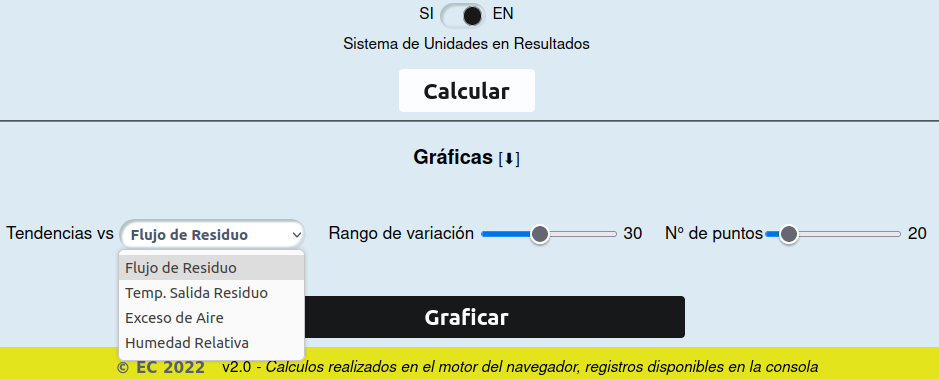
\includegraphics[scale=0.48]{images/curvas}
\caption[Opciones disponibles para graficar en el simulador]{Opciones disponibles para graficar en el simulador.}
\label{fig:curvas}\end{center}\end{figure}
\par Dependiendo del número de puntos escogidos por el usuario, el simulador podrá requerir más tiempo para finalizar los cálculos, en los rangos permitidos de la interfaz.
\par Definido un rango, este se divide entre un número de puntos establecido y se corre la simulación moviendo la variable escogida por cada punto.
\par Para visualizar los cambios generados se escogieron seis variables para ser graficadas, las cuales son:
\begin{enumerate}
    \item El flujo de combustible.
    \item La temperatura de arco radiante.
    \item La temperatura de chimenea.
    \item La relación de absorción de calor entre las zona radiante y la convectiva.
    \item La eficiencia térmica (@ Valor calorífico neto).
    \item Las emisiones de CO$_2$.
\end{enumerate}

\subsection{Variación de la carga del horno}
\par En la secuencia de Figuras \ref{fig:graph-t_out-fuel}, \ref{fig:graph-t_out-arc}, \ref{fig:graph-t_out-chim}, \ref{fig:graph-t_out-dist}, \ref{fig:graph-t_out-efic} y \ref{fig:graph-t_out-emi} se puede apreciar el cambio de las seis variables resultantes con la variación de la temperatura de salida del residuo (lo que es equivalente a aumentar la carga del horno), cuyas tendencias son equivalentes a aumentar el flujo de residuo de vacío.
\par Los puntos rojos representan los valores calculados por el simulador, unidos por una línea azul que representa su tendencia; en el rango del eje de las abscisas se presenta la variable de entrada escogida.
\par En la Figura \ref{fig:graph-t_out-fuel}, se grafica el flujo de combustible variando la temperatura del fluido. Se observa el incremento el flujo de combustible necesario para cumplir con el aumento de la carga del horno.
\begin{figure}[H]\begin{center}
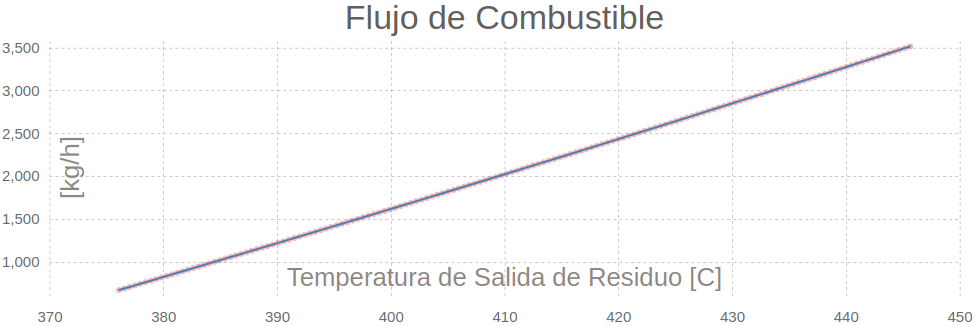
\includegraphics[scale=0.46]{images/graph-t_out-fuel}
\caption[Flujo de combustible en función de Temperatura de salida de residuo]{Flujo de combustible en función de la temperatura de salida de residuo.}
\label{fig:graph-t_out-fuel}\end{center}\end{figure}
\par Este comportamiento corresponde a que el combustible es la fuente de calor del horno y cualquier necesidad de energía adicional en el proceso requiere mayor flujo de combustible. Este comportamiento también se observa al aumentar el flujo de la carga, la humedad relativa y el exceso de aire, de forma independiente.
\par Al aumentar el flujo de combustible por el requerimiento de una temperatura de salida del fluido mayor, y manteniendo el resto de las variables de entrada, como exceso de aire y humedad relativa fijas, se nota un aumento en la temperatura de arco radiante (Fig. \ref{fig:graph-t_out-arc}) y, por consecuencia, en la temperatura de salida de los gases de chimenea (Fig. \ref{fig:graph-t_out-chim}).
\begin{figure}[H]\begin{center}
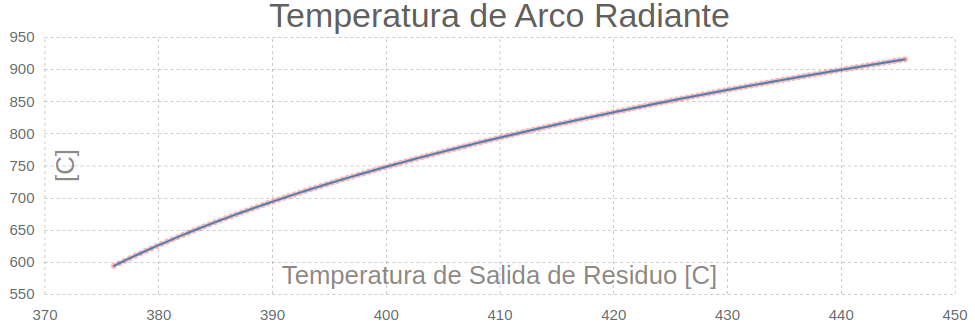
\includegraphics[scale=0.46]{images/graph-t_out-arc}
\caption[Temperatura de arco radiante en función de Temperatura de salida de residuo]{Temperatura de arco radiante en función de la temperatura de salida de residuo.}
\label{fig:graph-t_out-arc}\end{center}\end{figure}
\par El aumento observado en las Figuras \ref{fig:graph-t_out-fuel} y \ref{fig:graph-t_out-chim} se traduce en mas energía y gases de combustión liberados al ambiente, disminuyendo la eficiencia del horno y aumentado la contaminación generada por el proceso.
\begin{figure}[H]\begin{center}
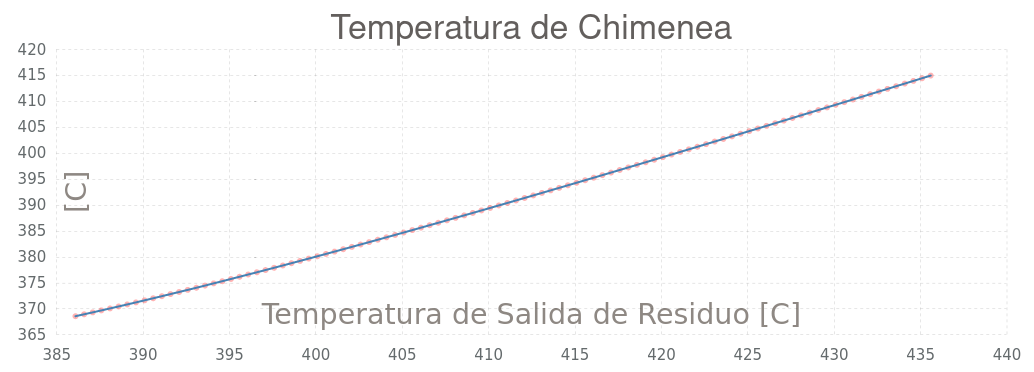
\includegraphics[scale=0.46]{images/graph-t_out-chim}
\caption[Temperatura de chimenea en función de Temperatura de salida de residuo]{Temperatura de chimenea en función de la temperatura de salida de residuo.}
\label{fig:graph-t_out-chim}\end{center}\end{figure}
\par Para la variable de la relación de calor absorbido por zona, la tendencia observada en la Figura \ref{fig:graph-t_out-dist} es decreciente, lo que se traduce en que el porcentaje de la absorción de calor disminuye en la zona radiante y aumenta en la zona convectiva, a pesar de que el calor transferido es siempre mayor en la zona radiante.
\begin{figure}[H] \begin{center}
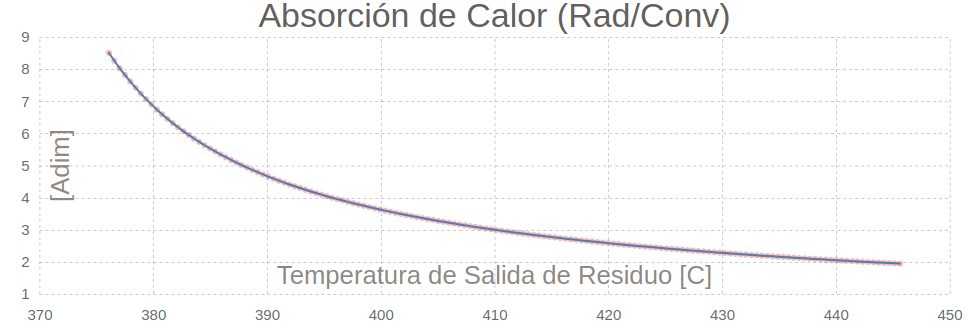
\includegraphics[scale=0.46]{images/graph-t_out-dist}
\caption[Distribución de absorción de calor en función de Temperatura de salida de residuo]{Tasa de distribución de absorción de calor entre zona radiante y convectiva en función de la temperatura de salida de residuo.}
\label{fig:graph-t_out-dist} \end{center} \end{figure}
\par Ambas zonas transfieren mayor cantidad de calor al fluido, pero la zona convectiva refleja un aumento porcentual mayor, proporcional a la temperatura de los gases de combustión, un factor a considerar es que la zona convectiva tiene un área de contacto casi diez veces mayor por la presencia de aletas.
\par Comprobando el comportamiento esperado de la eficiencia, se observa una tendencia decreciente en la Figura \ref{fig:graph-t_out-efic}, al aumentar cualquiera de las variables de entrada seleccionadas para este análisis, un comportamiento inversamente proporcional al aumento de la temperatura de los gases en la chimenea.
\begin{figure}[H]\begin{center}
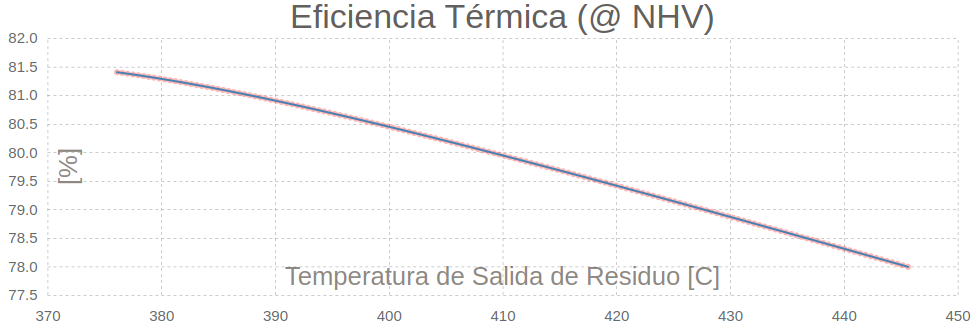
\includegraphics[scale=0.46]{images/graph-t_out-efic}
\caption[Eficiencia térmica en función de Temperatura de salida de residuo]{Eficiencia Térmica (@ Valor Calorífico Neto) en función de la temperatura de salida de residuo.}
\label{fig:graph-t_out-efic}\end{center}\end{figure}
\par La tendencia al incremento del flujo de combustible que se observa para todas las variables estudiadas, es directamente proporcional a las emisiones de dióxido de carbono, lo que puede corroborarse en la Figura \ref{fig:graph-t_out-emi}.
\begin{figure}[H] \begin{center}
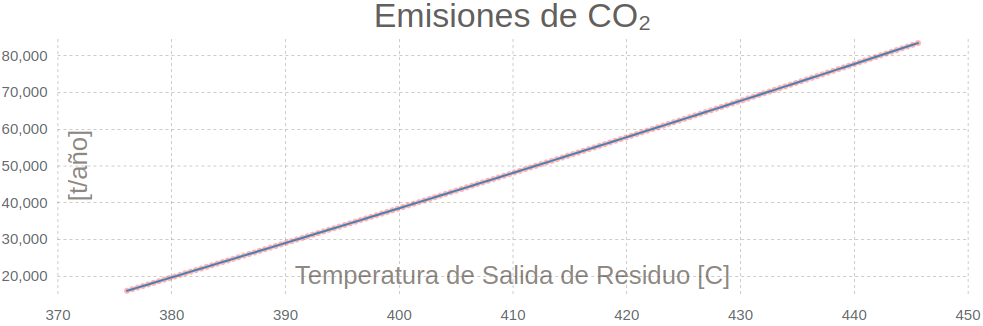
\includegraphics[scale=0.46]{images/graph-t_out-emi}
\caption[Emisiones de CO$_2$ en función de Temperatura de salida de residuo]{Emisiones de CO$_2$ en función de la temperatura de salida de residuo.}
\label{fig:graph-t_out-emi} \end{center} \end{figure}

\subsection{Variación del exceso de aire y humedad relativa}
\par Para la variable del exceso de aire se observan las mismas tendencias de aumento del flujo de combustible, temperatura de chimenea y emisiones de CO$_2$; y tendencias de disminución de la eficiencia térmica y del porcentaje de absorción de calor en la zona radiante.
\begin{figure}[H] \begin{center}
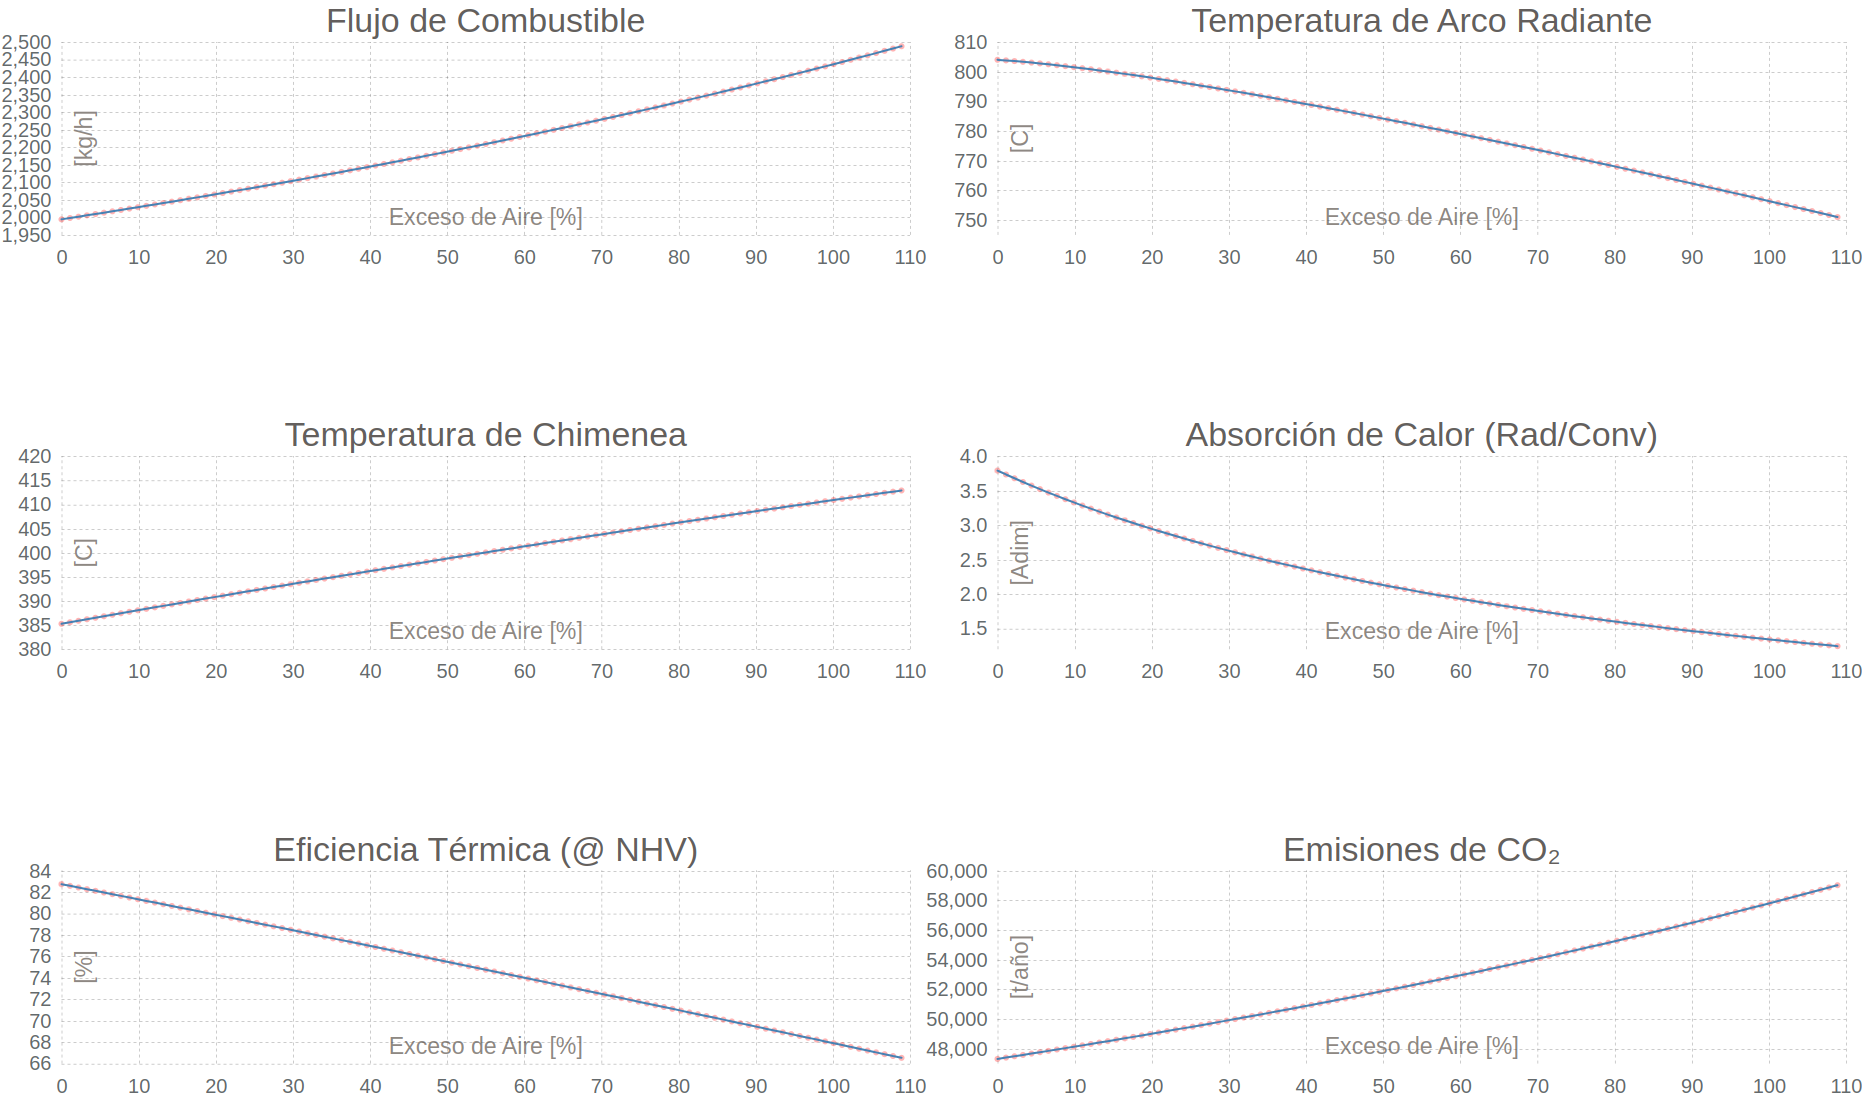
\includegraphics[scale=0.24]{images/exceso-aire}
\caption[Curvas de tendencia para la variación de exceso de aire]{Curvas de tendencia para la variación de exceso de aire.}
\label{fig:exceso-aire} \end{center} \end{figure}
\par Observando que la única tendencia diferente es la correspondiente a la temperatura de arco radiante, que disminuye al aumentar el flujo másico de los gases de combustión, a causa de un consumo de calor adicional en calentar el exceso de aire en la cámara de combustión, como se aprecia en la ecuación de temperatura de arco, descrita en la sección de combustión de hidrocarburos.
\par Comportamiento y tendencias similares se observan cuando se varia la humedad relativa en el aire de alimentación. Con lo que se tiene una referencia de la tendencia en todas las variables abiertas para graficar.

\section{Resultados del modo comparativo}
\par Este modo permite ver en paralelo dos estados distintos del horno, uno base y otro modificado, lo que posibilita comparar los cambios en las variables resultantes del proceso y analizar las causas de estos cambios. Se aconseja modificar solo una variable de entrada en cada comparación para un análisis específico.
\par En la Tabla \ref{tbl:comparison-cp} se observa un resumen de las condiciones de operación por comparar, un caso base frente a una modificación del combustible; ambos combustibles son gases de refinería con la particularidad que el modificado tiene 4 veces más hidrógeno que el caso base y, proporcionalmente, menos hidrocarburos.
\par En la Tabla \ref{tbl:comparison-r} se detallan uno a uno los resultados del caso base y modificado, de manera semejante a como se muestra en la interfaz web. Dentro de los resultados para esta comparación se resalta la disminución, tanto del flujo de combustible en un 3.5\%, como de las emisiones de CO$_2$ en un 10.8\%; lo que se debe directamente a disminuir el uso de hidrocarburos en el combustible del horno.

\begin{table}[H]
\caption{Condiciones de proceso del modo comparativo del simulador}
\label{tbl:comparison-cp}
\centering
\begin{tabular}{l|c|c}
CASO    & BASE & MODIFICADO \\

\multicolumn{3}{c}{Residuo atmosférico} \\
Flujo volumétrico,  m$^3$/d      &14,309 &14,309 \\
Temperatura de entrada,  °C   &359    &359    \\
Temperatura de salida,  °C    &411    &411    \\
Gravedad específica           &0.84   &0.84   \\
Calor absorbido total,  MW    &20.862 &20.862 \\
\multicolumn{3}{c}{Factores de ensuciamiento} \\
Rfi (interno) radiante,  m$^2$-K/W 10$^{-3}$        &0.100  &0.100 \\
Rfi interno escudo/convectivo,  m$^2$-K/W 10$^{-3}$ &0.100  &0.100 \\
Rfo externo escudo/convectivo,  m$^2$-K/W 10$^{-3}$ &0.100  &0.100 \\

\multicolumn{3}{c}{Condiciones de combustión} \\
Exceso de aire, \%                      &20     &20   \\
Temperatura del aire de combustión, °C  &27     &27   \\
Humedad relativa, \%                    &50     &50   \\
Humedad del aire,  gH$_2$O/kg aire seco &11.107 &11.107 \\
Pérdidas de calor al ambiente, \%  &1.5    &1.5  \\

\multicolumn{3}{c}{Características del combustible} \\
Metano (CH$_4$), \%          &56.47  &30.47  \\
Etano (C$_2$H$_6$), \%       &15.15  &8.15   \\
Propano (C$_3$H$_8$), \%     &6.22   &5.22   \\
n-Butano (C$_4$H$_{10}$), \% &1.76   &1.50   \\
i-Butano (C$_4$H$_{10}$), \% &0.75   &0.75   \\
Etileno (C$_2$H$_4$), \%     &1.58   &1.58   \\
Propileno (C$_3$H$_6$), \%   &2.77   &2.77   \\
Monóxido de carbono (CO), \% &0.66   &0.66   \\
Hidrógeno (H$_2$), \% &11.42&\colorbox{lightgray}{45.68}\\
Nitrógeno (N$_2$), \%        &0.68   &0.68   \\
Dióxido de carbono (CO$_2$), \%&2.54 &2.54   \\
\hline
Peso molecular,  kg/kmol               &21.149 &14.972 \\
Calor específico Cp (T comb),  kJ/kg-K &3.410  &7.595  \\
Poder Calorífico Neto (NCV),  kJ/kg    &45.718 &47.680 \\
Poder Calorífico Bruto (GCV),  kJ/kg   &50.268 &52.814 \\
\end{tabular}
\end{table}

\begin{table}[H]
\caption{Resultados del modo comparativo del simulador}
\label{tbl:comparison-r}
\centering
\begin{tabular}{l|c|c}
\text{    } CASO & BASE & MODIFICADO \\
\multicolumn{3}{c}{Flujos másicos,  kg/s} \\
Fluido de proceso (Residuo atmosférico)   &139.0         &139.0  \\
Combustible           &0.57 &\colorbox{lightgray}{0.55} \\
Aire                  &10.68         &10.38  \\
Gases de combustión   &11.28         &10.92  \\
\hline
(A/C) Masa BH        &18.693 &19.034 \\
(A/C) Volumen BH     &13.795 &9.944  \\
\hline
Suministro Térmico Combustible,  MW  &26.118 &25.999 \\
Suministro Térmico Total,  MW        &26.266 &26.169 \\
\hline
\multicolumn{3}{c}{Calor Absorbido,  MW}\\
Sección Radiante - (\%)  &13.099 - (62.79) &13.185 - (63.20)\\
Sección Escudo - (\%)    &3.311 - (15.87)  &3.313 - (15.88) \\
Sección Convectiva - (\%)&4.441 - (21.29)  &4.353 - (20.87) \\
\hline
Temperatura de pared (tubos radiantes), °C &434  &434  \\
Temperatura de Arco radiante, °C         &798  &798  \\
Temperatura de Chimenea, °C              &391  &391  \\
Temperatura Máxima Aletas (perímetro), °C &377  &376  \\
\hline
\multicolumn{3}{c}{Análisis de gases de combustión (Base Húmeda)}\\
CO$_2$, \%     &8.72    &7.93    \\
N$_2$, \%      &71.84   &71.23   \\
O$_2$, \%      &3.17    &3.14    \\
H$_2$O, \%     &16.27   &17.70   \\
\hline
Emisiones de CO$_2$, tonelada/año &48.790  &\colorbox{lightgray}{43.523} \\
\hline
\multicolumn{3}{c}{Pérdidas de calor,  MW}\\
Por chimenea - (\% del total)&4.888 - (18.61) &4.796 - (18.33) \\
Al ambiente - (\% del total) &0.392 - (1.49)  &0.390 - (1.49) \\
\hline
Eficiencia Térmica @ NHV, \%  &79.90 &80.18 \\
%Eficiencia Térmica @ GHV, \%  &72.70 &72.43 \\
\end{tabular}
\end{table}

\par Otra comparación, al modificar únicamente el exceso de aire, de un 20\% a un 40\%, se observa: aumento en el consumo de combustible en un 3.4\%, aumento en las emisiones de CO$_2$ en un 3.6\%, aumento en el flujo de gases de combustión en un 16.9\% y disminución en la eficiencia térmica de un 3.0\%. Esto debido a que el horno pierde energía al calentar el exceso de aire que se ingresa para la combustión, evidenciando la importancia de esta variable en el proceso.

% 6-      No existe impedimento para variar el fluido del proceso en un amplio margen de crudos con diferentes API u otras corrientes de refinería.